\documentclass[11pt,a4paper]{article}

% =============================
% Packages
% =============================
\usepackage[margin=0.85in]{geometry}
\usepackage{setspace}
\usepackage{graphicx}
\usepackage{booktabs}
\usepackage{longtable}
\usepackage{tabularx}
\usepackage{array}
\usepackage{float}
\usepackage{xcolor}
\usepackage{fancyhdr}
\usepackage{titlesec}
\usepackage{caption}
\usepackage{hyperref}
\usepackage{makecell}
\usepackage{multicol}
\usepackage{ragged2e}
\usepackage{siunitx}

% =============================
% Document formatting
% =============================
\onehalfspacing
\hypersetup{colorlinks=true, linkcolor=black, urlcolor=blue}
\setlength{\parskip}{0.55em}
\setlength{\parindent}{0pt}
\renewcommand{\arraystretch}{1.18}
\newcolumntype{Y}{>{\raggedright\arraybackslash}X}

% =============================
% Section formatting
% =============================
\titleformat{\section}{\Large\bfseries}{\thesection}{0.7em}{}
\titleformat{\subsection}{\large\bfseries}{\thesubsection}{0.7em}{}

% =============================
% Footer/Header for subsequent pages
% =============================
\pagestyle{fancy}
\fancyhf{}
\fancyhead[L]{9 August 2026}
\fancyhead[R]{Generated by LAMBDA: \url{https://lambda.com.ai}}
\cfoot{\thepage}
\renewcommand{\headrulewidth}{0.4pt}

% =============================
% First page custom header
% =============================
\fancypagestyle{firstpage}{
    \fancyhf{}
    \fancyhead[L]{%
        \raisebox{-0.5\height}{
\includegraphics[height=1.5cm]{res/logo.png}}
        \\[0.8em]
        \rule{\textwidth}{0.6pt}
    }
    \cfoot{\thepage}
    \renewcommand{\headrulewidth}{0pt}
}

\begin{document}
\thispagestyle{firstpage}

\begin{center}
  \vspace*{3cm}
  {\LARGE \textbf{Pulmonary Hypertension Services in Great Britain\\The NAPH 10th Annual Report -- Key Findings and Survival Analysis}} \\[0.5em]
  {\large LAMBDA} \\[0.5em]
  {\large 9 August 2026}
\end{center}

\begin{abstract}
This analysis examines the National Audit of Pulmonary Hypertension (NAPH) 10th Annual Report covering 2018--19 data from eight specialist pulmonary hypertension centres across England, Scotland, and Wales. The report evaluates clinical care quality against 13 national standards, analyses survival outcomes for over 4,800 IPAH patients diagnosed since 2009, and reviews local action plans from participating centres. Eleven of 13 national standards were met at a national level, demonstrating substantial improvement in diagnosis timeliness, cardiac catheterisation compliance, and quality-of-life recording. However, two critical areas remain unresolved: only 11\% of CTEPH patients received pulmonary endarterectomy within four months (target 90\%), and vasoreactivity testing was recorded for only 57\% of eligible IPAH patients. Survival curves reveal stark differences by comorbidity status, age, sex, and WHO functional class, with IPAH patients without comorbidities achieving 80\% five-year survival compared to just 25\% for those with comorbidities.
\end{abstract}

\newpage

\section{The patient load is growing faster than capacity}

The number of active PH patients managed by UK specialist centres grew from 4,341 in 2010 to 8,351 in 2019 -- a 92\% increase over nine years. Active drug therapies increased even more sharply, from 2,400 to 4,700, reflecting both disease expansion and therapeutic intensification. Sheffield alone added 1,236 active patients over this period, growing from 947 to 2,183, while Royal Free nearly tripled from 629 to 1,774. Golden Jubilee saw the steepest proportional rise, increasing its caseload from 350 to 669 (+91\%).

Royal Papworth, the single UK centre for pulmonary endarterectomy (PEA), now manages 1,190 active patients -- up 69\% from 705 in 2010. Its patient volume exceeds Imperial College (1,034) and is second only to Sheffield (2,183) among adult centres. These volumes are sustained above the raised standard of 300 PAH/CTEPH patients per year set for every adult centre, confirming that workload thresholds derived from ESC/ERS guidelines continue to be conservative relative to actual demand.

\begin{table}[H]
\centering
\small
\caption{Active patients on 31 March by PH centre (selected years)}
\begin{tabularx}{\textwidth}{lrrr@{}l}
\toprule
PH Centre & 2010 & 2014 & 2019 & Growth 2010--19 \\
\midrule
Sheffield & 947 & 1,458 & 2,183 & +131\% \\
Royal Free & 629 & 905 & 1,774 & +182\% \\
Royal Papworth & 705 & 964 & 1,190 & +69\% \\
Imperial College & 650 & 874 & 1,034 & +59\% \\
Royal Brompton \& Harefield & 502 & 691 & 829 & +65\% \\
Golden Jubilee & 350 & 498 & 669 & +91\% \\
Newcastle & 280 & 316 & 361 & +29\% \\
Great Ormond Street & 278 & 301 & 311 & +12\% \\
\textbf{Total} & \textbf{4,341} & \textbf{5,007} & \textbf{8,351} & \textbf{+92\%} \\
\bottomrule
\end{tabularx}
\end{table}

The sustained growth has operational implications: the median time from CTEPH diagnosis to PEA surgery stood at 26 weeks in 2018--19, marginally improved from 29 weeks in 2017--18 but still far exceeding the four-month target. Royal Papworth's leadership team explicitly attributes limited surgical throughput to the hospital relocation in 2019, noting that the new facility will enable increased operations. Until then, the bottleneck will persist regardless of referral efficiency improvements at sending centres.

\begin{figure}[H]
  \centering
  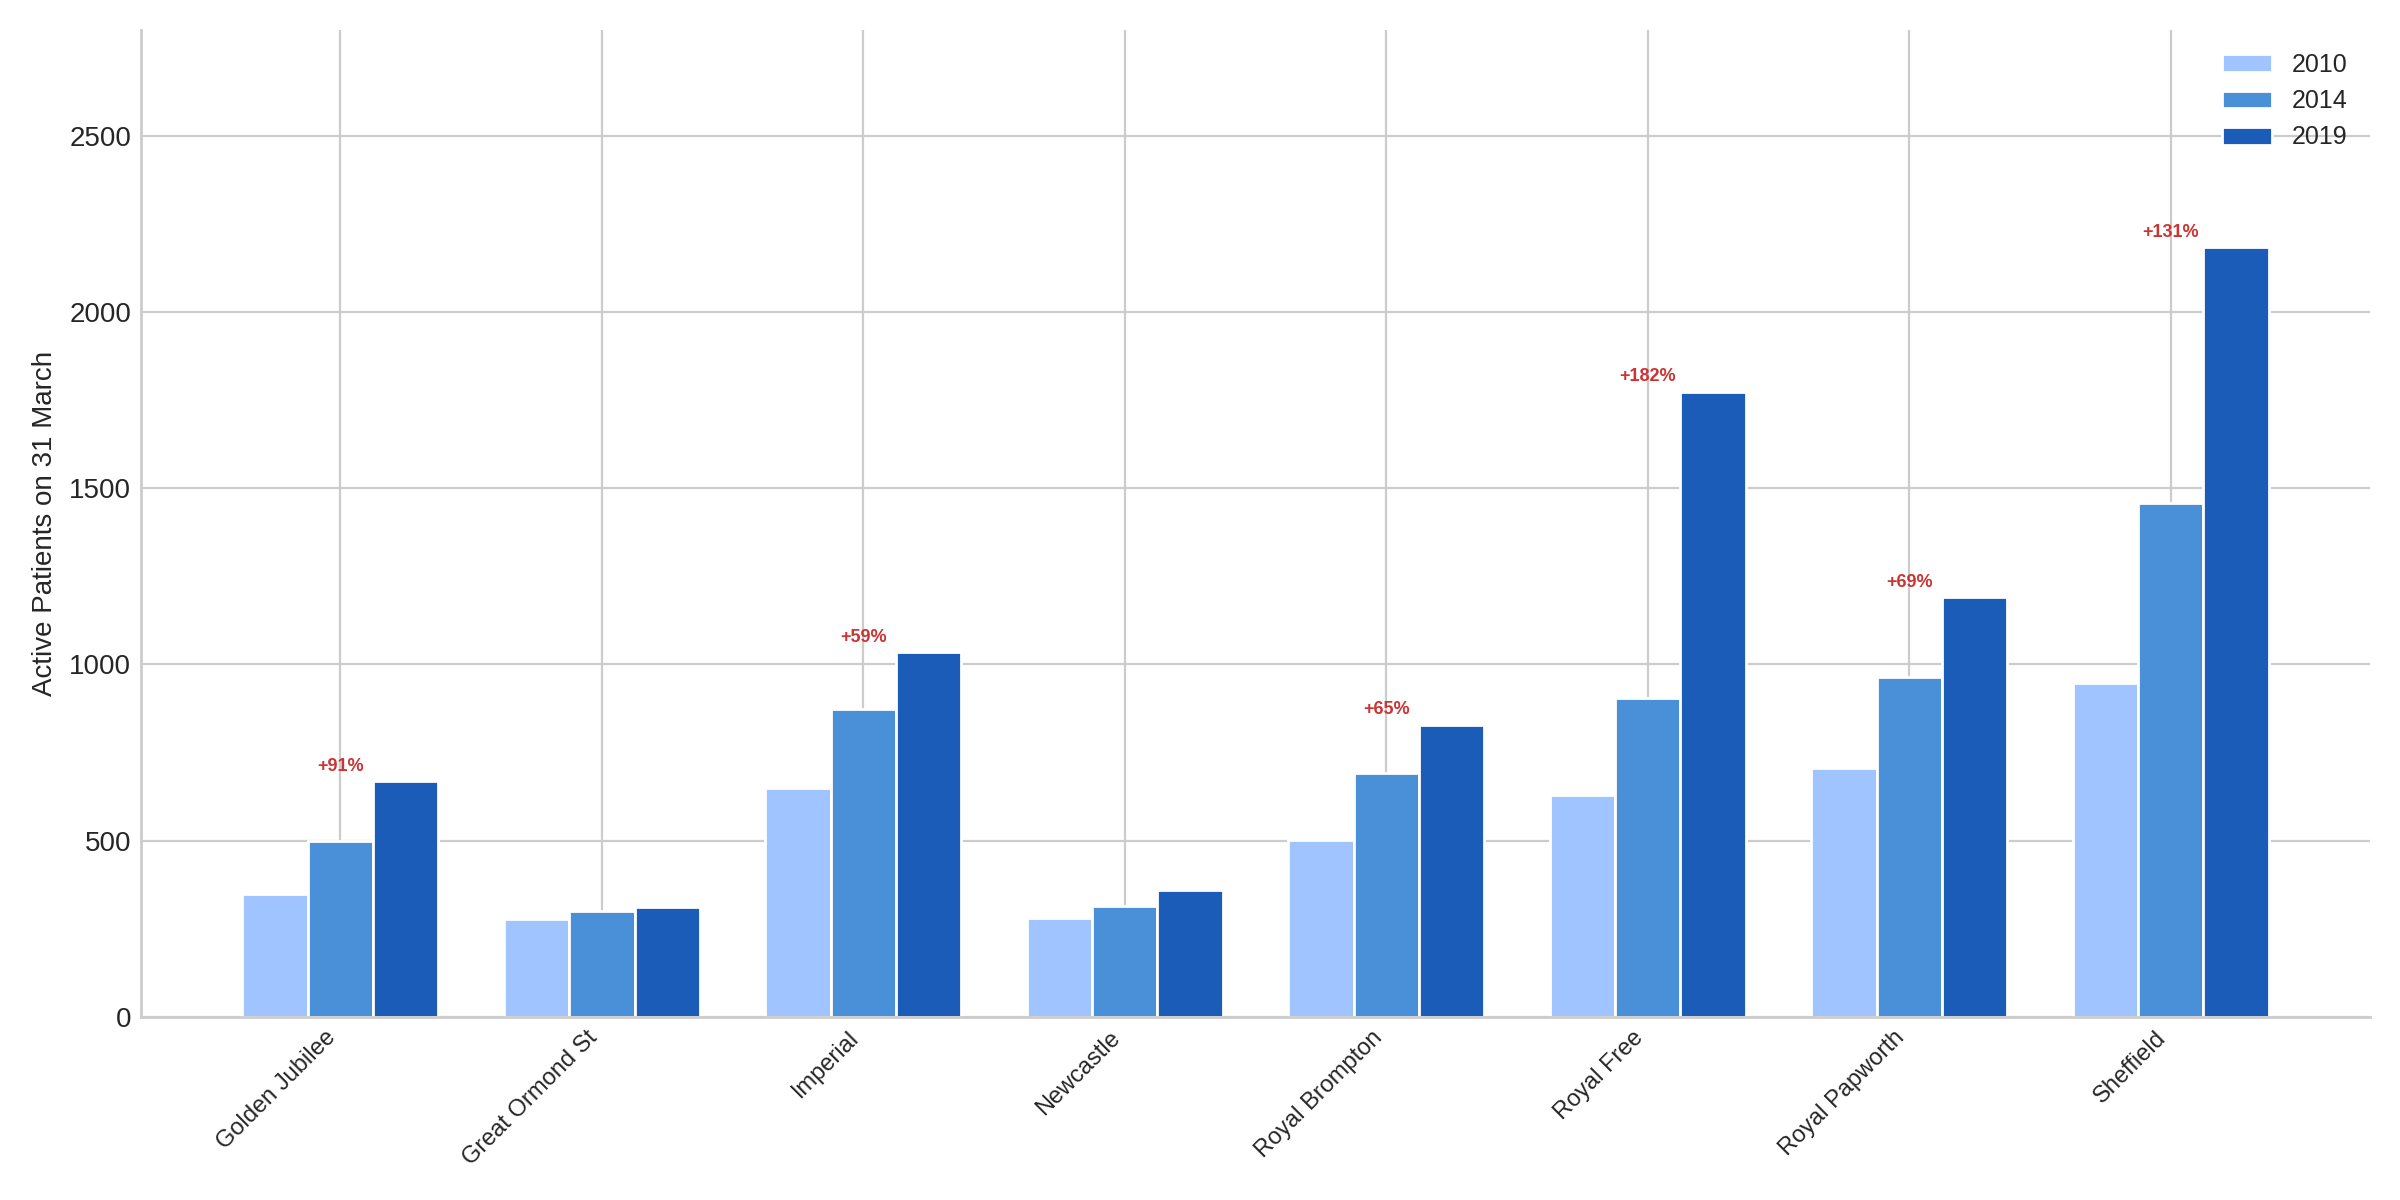
\includegraphics[width=\textwidth]{chart_patient_volumes.png}
  \caption{Active patient volumes rose steeply at most centres between 2010 and 2019. Sheffield led absolute growth; Royal Free showed the highest proportional increase. Source: NAPH Reference Table R1.}
\end{figure}

\section{Most process standards have converged toward targets}

At the national level, eleven of thirteen standards were met in 2018--19. The trajectory of achievement reveals clear improvement patterns since 2015--16 when data collection became systematic. Four standards show statistically significant upward trends: timely diagnosis (NS3, up to 99\%), being seen within 30 days (NS4, up to 63\%), pre-treatment cardiac catheterisation (NS5, up to 97\%), and vasoreactivity study recording (NS7, new at 57\%). Three others plateaued at high levels -- annual consultation (NS12 at 96\%), quality-of-life recording (NS11 at 96\%), and PDE5 first-line therapy (NS10 at 91\%). Two reached near-perfect attainment long ago: participation (NS1, 8 of 8 centres) and diagnosis recording for patients on drugs (NS9, 100\%).

The most remarkable improvement occurred in Standard 4 (seen or discharged within 30 days), which rose from 47\% in 2015--16 to 63\% in 2018--19, becoming the first standard where all centres met the threshold simultaneously. Newcastle's leap from 19\% to 78\% was the largest single-centre gain on this measure. Royal Brompton credited this progress to bi-monthly data analysis against standards and continuous error correction by their data entry manager.

Two standards remain problematic. NS13 (PEA waiting times under four months) has never been met nationally; it fell further from 18\% in 2017--18 to 11\% in 2018--19. Six out of seven reporting centres achieved zero to ten percent compliance. Meanwhile, NS7 (vasoreactivity studies before treatment) was introduced at the 80\% target and recorded at just 57\%, suggesting that centres need time to embed the new measurement into clinical pathways.

\begin{figure}[H]
  \centering
  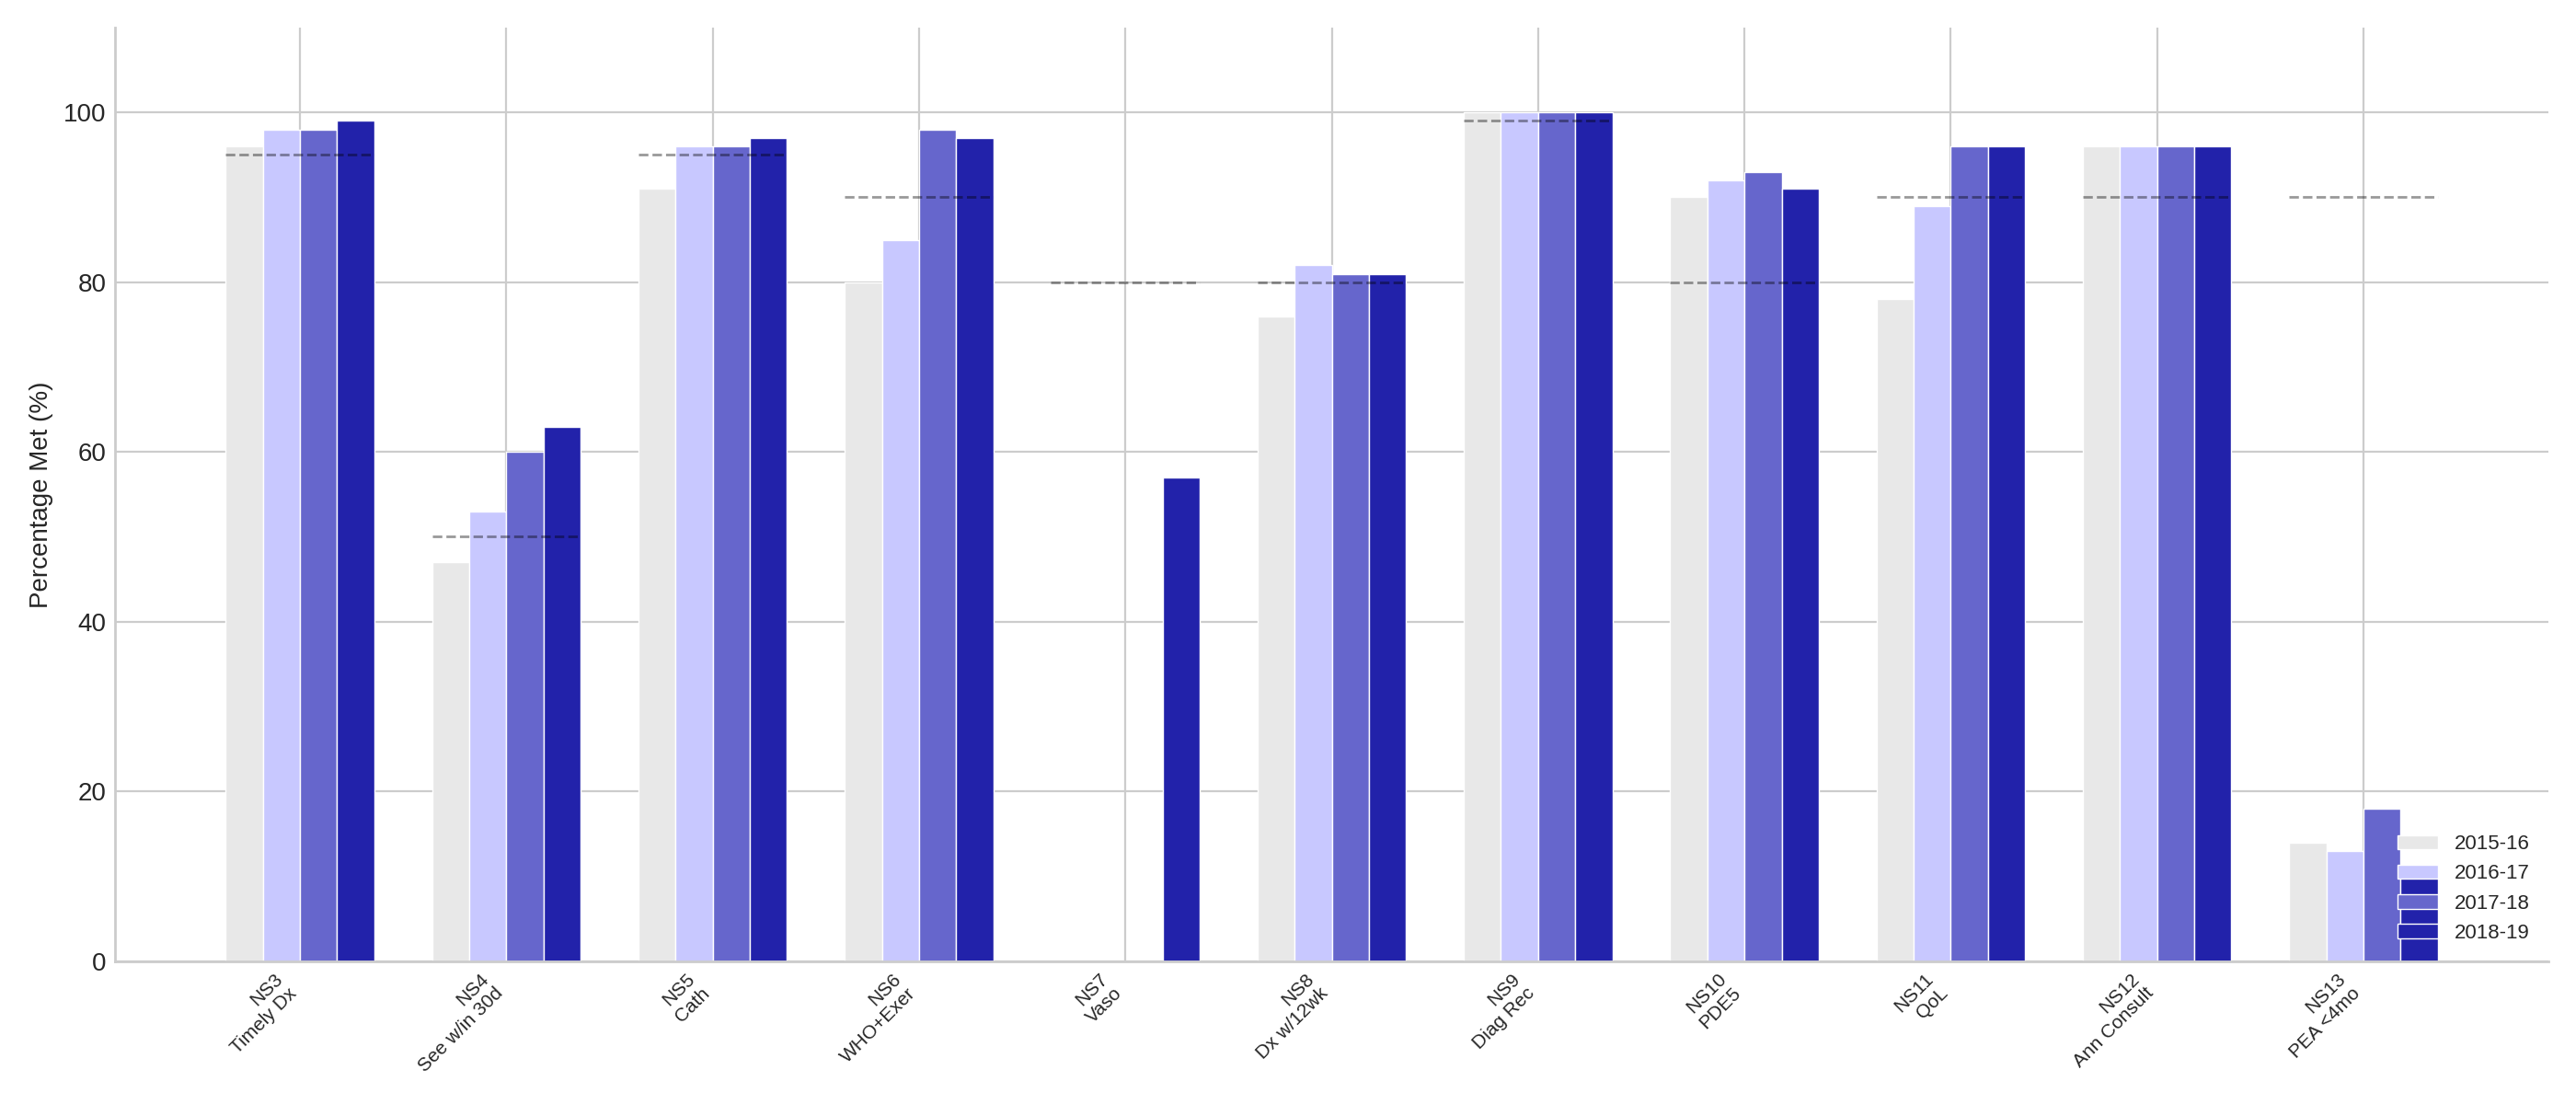
\includegraphics[width=\textwidth]{chart_standards_trends.png}
  \caption{Trends in national standards compliance from 2015--16 to 2018--19. Dashed horizontal lines indicate targets. Only 11 of 13 standards were met at the national level in 2018--19. NS4 shows the steepest improvement; NS13 remains persistently below target.}
\end{figure}

\begin{figure}[H]
  \centering
  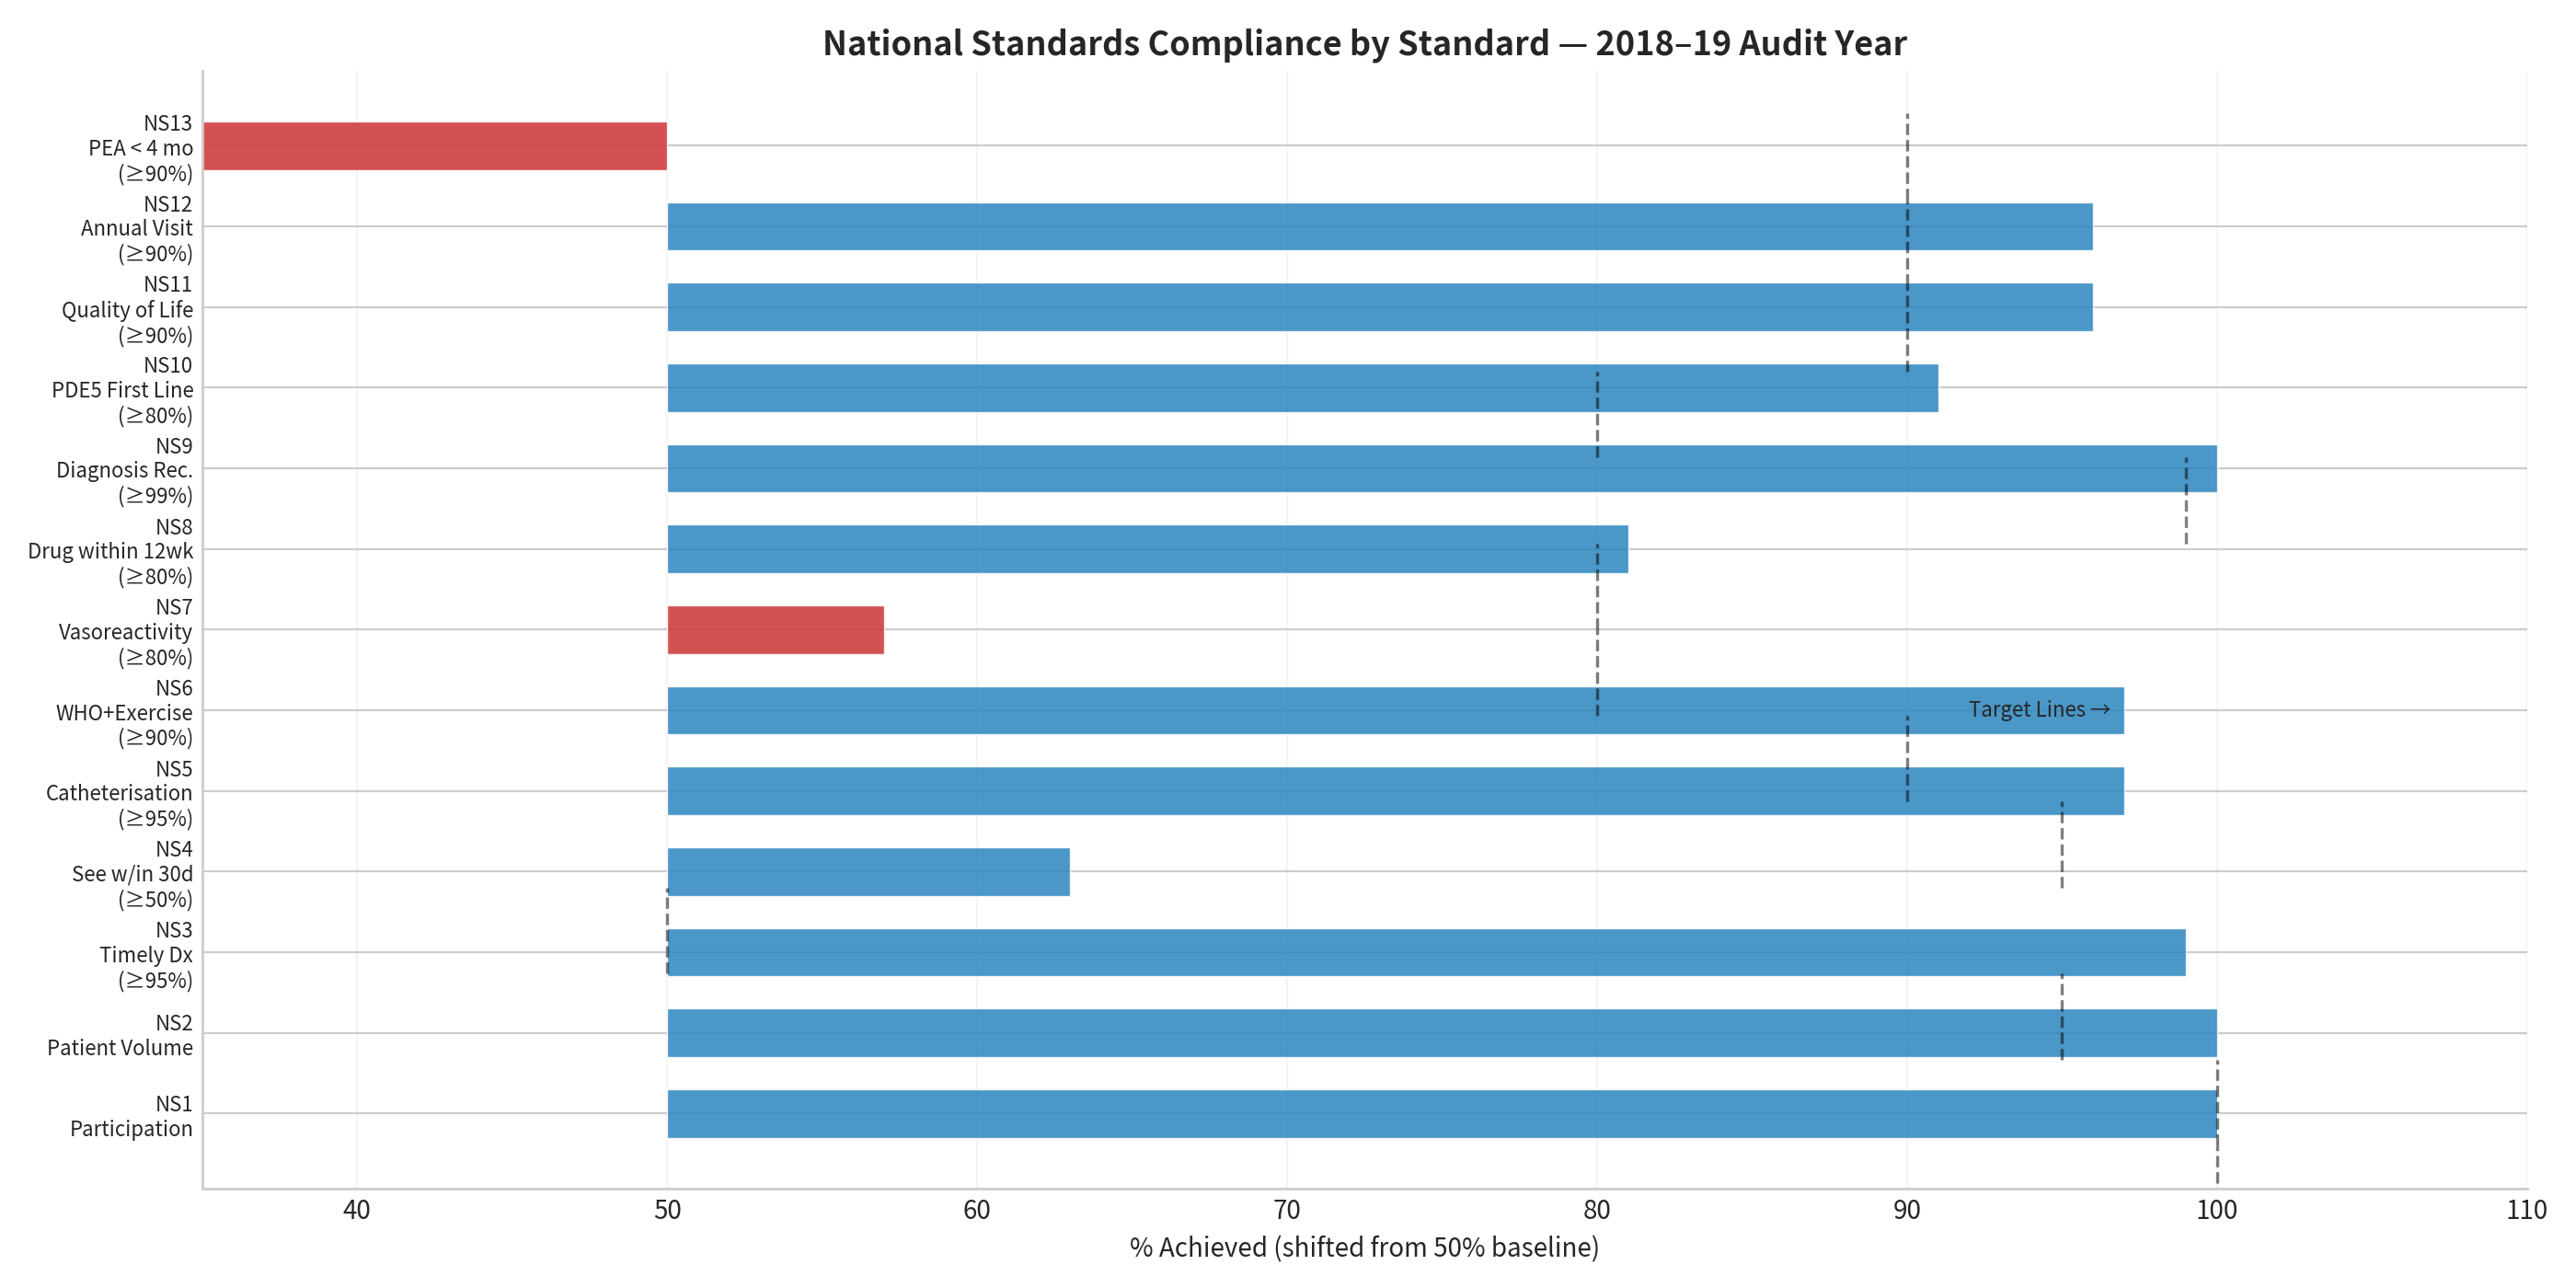
\includegraphics[width=\textwidth]{chart_standards_horizontal.png}
  \caption{Performance against each national standard in 2018--19. Standards marked in red fall below their target. NS13 stands as the most severe gap, with only 11\% meeting the 90\% target for PEA waiting times.}
\end{figure}

Centre-level variation warrants scrutiny. Every centre misses at least one standard, meaning no organisation delivers uniformly high-quality care. Royal Papworth's strong performance on NS3 (timely diagnosis, 99\%) and NS5 (cardiac catheterisation, 97\%) contrasts with its poor showing on NS4 (only 53\% seen within 30 days), a paradox explained by the centre's own note that patients are discussed sooner at PEA MDT meetings but surgery volume did not increase during relocation. Conversely, Imperial College and Newcastle achieved perfect NS9 scores (diagnosis recorded) and strong NS5 results despite lower NS4 performance.

\begin{table}[H]
\centering
\small
\caption{Centre performance on key variable standards (2018--19)}
\resizebox{\textwidth}{!}{%
\begin{tabular}{lcccccc}
\toprule
PH Centre & NS3 Dx & NS4 See 30d & NS5 Cath & NS8 Drug 12wk & NS11 QoL & NS13 PEA <4mo \\
\midrule
Sheffield & 100\% & 55\% & 98\% & 79\% & 99\% & 6\% \\
Royal Papworth & 99\% & 53\% & 97\% & 75\% & 93\% & 23\% \\
Imperial College & 100\% & 62\% & 92\% & 89\% & 95\% & 10\% \\
Royal Free & 99\% & 75\% & 97\% & 87\% & 98\% & 0\% \\
Newcastle & 94\% & 78\% & 100\% & 91\% & 100\% & 0\% \\
Royal Brompton & 99\% & 57\% & 97\% & 88\% & 93\% & 0\% \\
Golden Jubilee & 99\% & 74\% & 99\% & 61\% & 94\% & 23\% \\
Great Ormond St & 89\% & 100\% & N/A & N/A & N/A & N/A \\
\textbf{National} & \textbf{99\%} & \textbf{63\%} & \textbf{97\%} & \textbf{81\%} & \textbf{96\%} & \textbf{11\%} \\
\textbf{Target} & \textbf{95\%} & \textbf{50\%} & \textbf{95\%} & \textbf{80\%} & \textbf{90\%} & \textbf{90\%} \\
\bottomrule
\end{tabular}%
}
\end{table}

\section{Comorbidities dominate IPAH survival prognosis}

Survival analysis represents the audit's most clinically valuable output. It draws on the longitudinal cohort of adult patients whose first referral was on or after 1 April 2009, using mortality data submitted directly by PH centres supplemented by Office for National Statistics records. Scottish patients at Golden Jubilee cannot be traced at ONS due to pseudonymisation, limiting inclusion in lung disease and left heart disease survival analyses.

Following a comprehensive review of all IPAH diagnoses conducted in early 2019, patients were reclassified as having IPAH with or without significant comorbid conditions (other cardiac, circulatory, or respiratory disease). This subdivision dramatically clarifies outcome expectations. Of the 2,077 IPAH patients in the refined dataset, 1,657 (69\%) were classified as IPAH without comorbidities and 420 as IPAH with comorbidities. An additional 321 patients previously coded as IPAH were reclassified into other diagnostic groups (lung disease, left heart disease, etc.), and 185 received corrected IPAH classifications.

\begin{figure}[H]
  \centering
  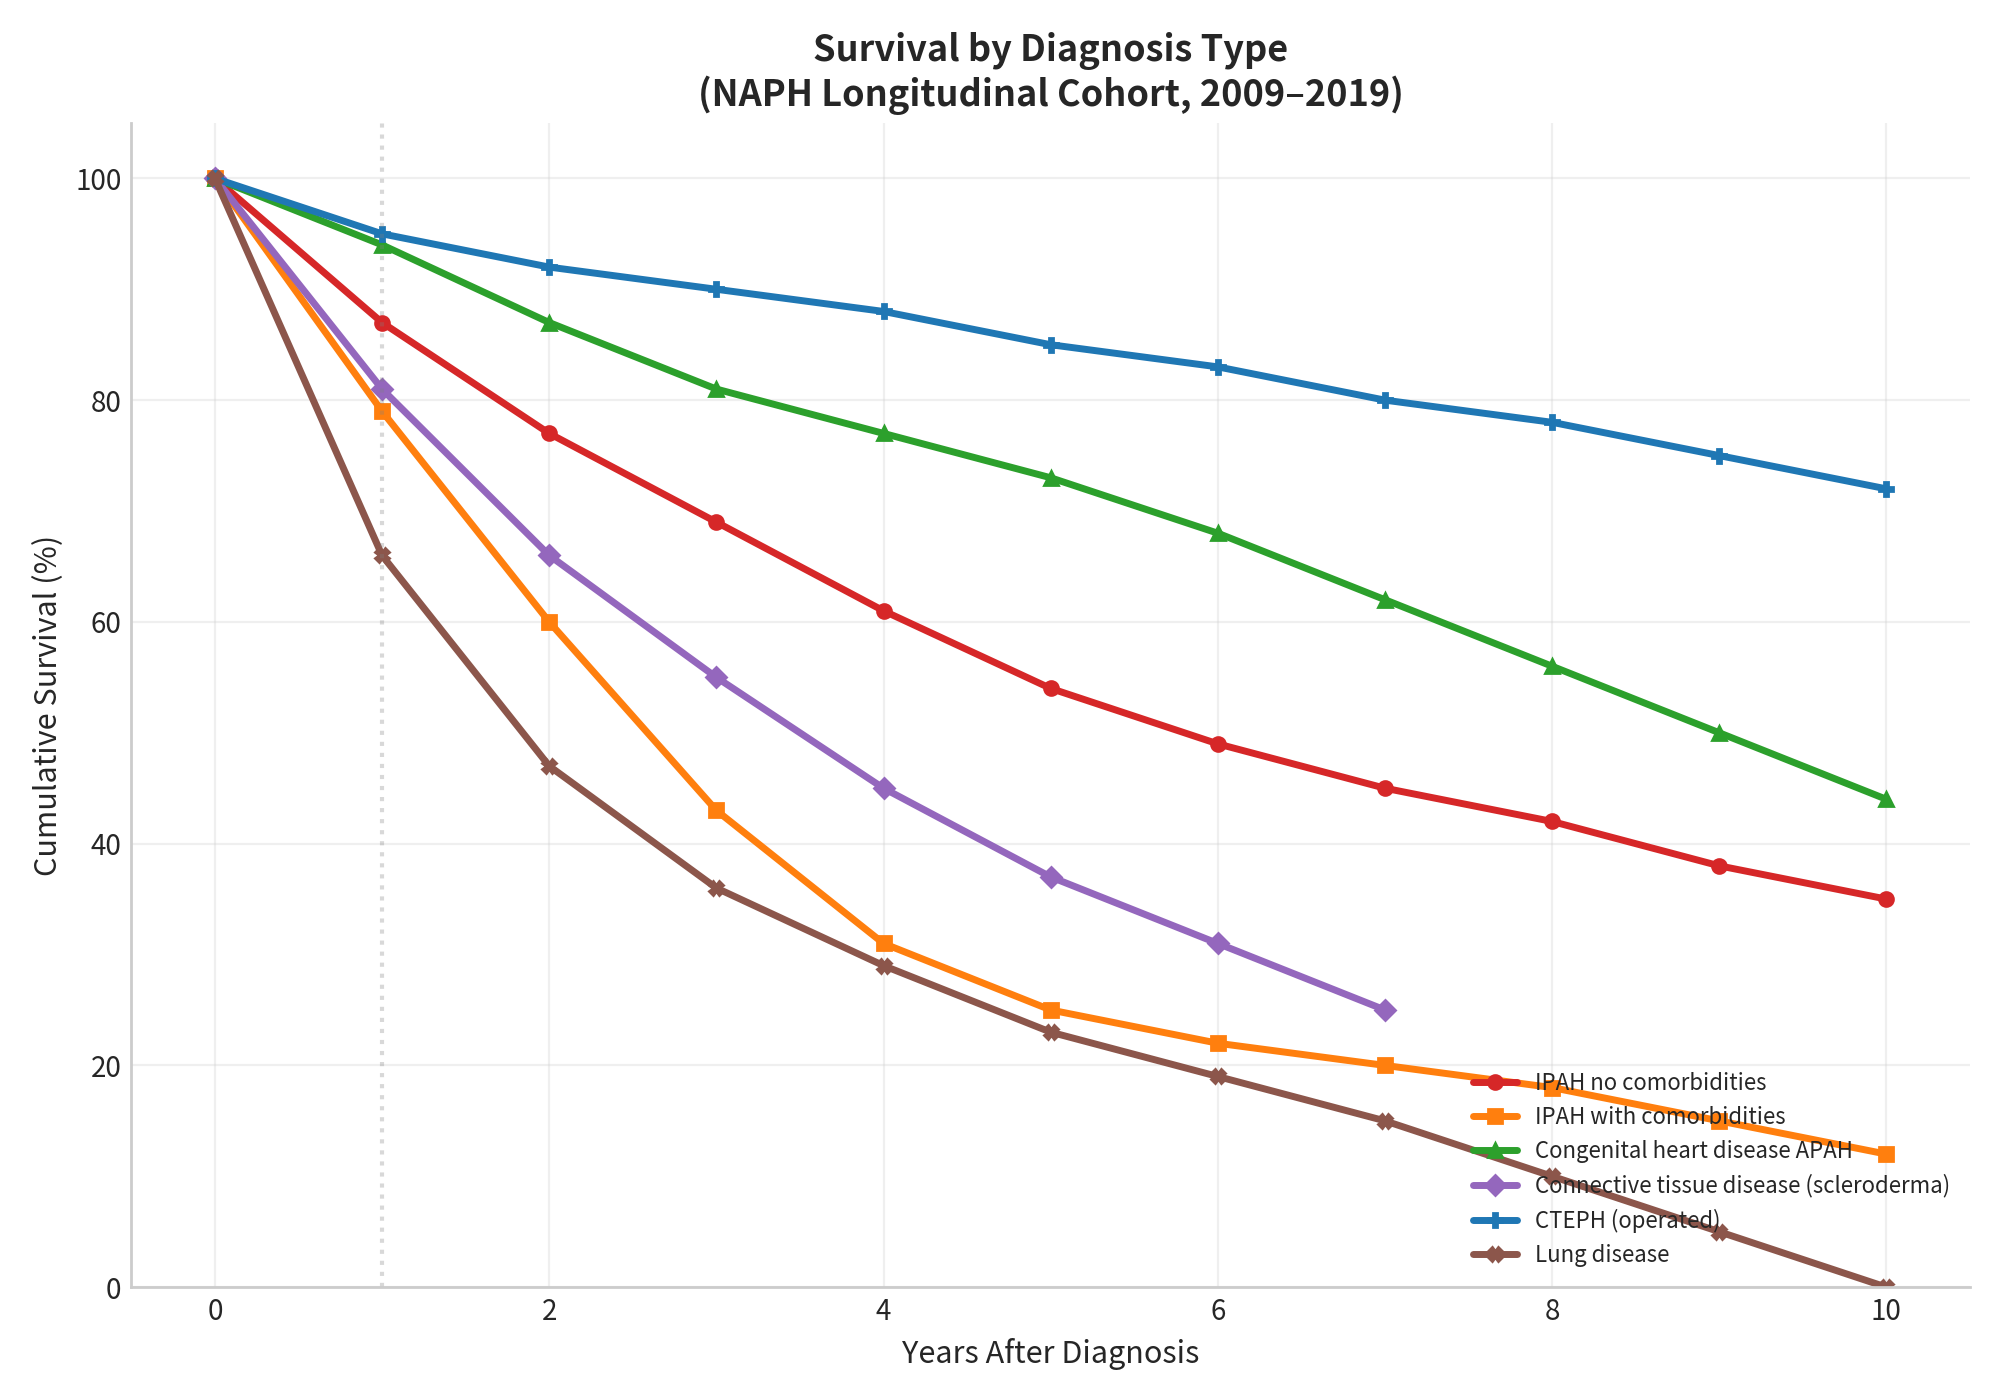
\includegraphics[width=\textwidth]{chart_survival_diagnosis.png}
  \caption{Cumulative survival curves by primary diagnosis type. IPAH without comorbidities achieves approximately 35\% survival at 10 years, whereas those with comorbidities drop to 12\%. Operated CTEPH patients achieve the best prognosis at 72\%. Lung disease carries the worst outlook, with near-zero survival beyond eight years.}
\end{figure}

For IPAH patients without comorbidities, five-year cumulative survival stands at 54\% (880 patients alive at one year from an initial 1,132). By contrast, IPAH patients with comorbidities reach only 43\% at three years (down from 100\% baseline with 385 patients), and five-year data is unavailable because fewer than 50 patients remain in the denominator. The divergence between the two curves becomes statistically significant at approximately 207 days from diagnosis.

The 2019 IPAH review had a measurable effect on reported survival: IPAH patients overall (before splitting by comorbidities) improved from 54\% five-year survival in the 9th AR (based on 1,645 mixed patients) to 50\% in the 10th AR (1,517 patients including comorbidities), but the isolated IPAH-without-comorbidities subgroup reaches 54\% -- suggesting that the previous composite curve suppressed true IPAH prognosis by mixing in sicker patients misattributed to the IPAH category.

Age exerts equally powerful effects. Patients in the youngest quintile (18--41 years, n=227) show exceptional survival: 90\% at three years and 84\% at five years, with 50\% mortality not yet reached at six years and 218 days. By comparison, patients aged 74--91 exhibit 46\% survival at three years and 30\% at five years. The oldest group's median post-diagnosis mortality occurs at 2 years and 291 days -- less than half the span of the youngest quintile.

\begin{figure}[H]
  \centering
  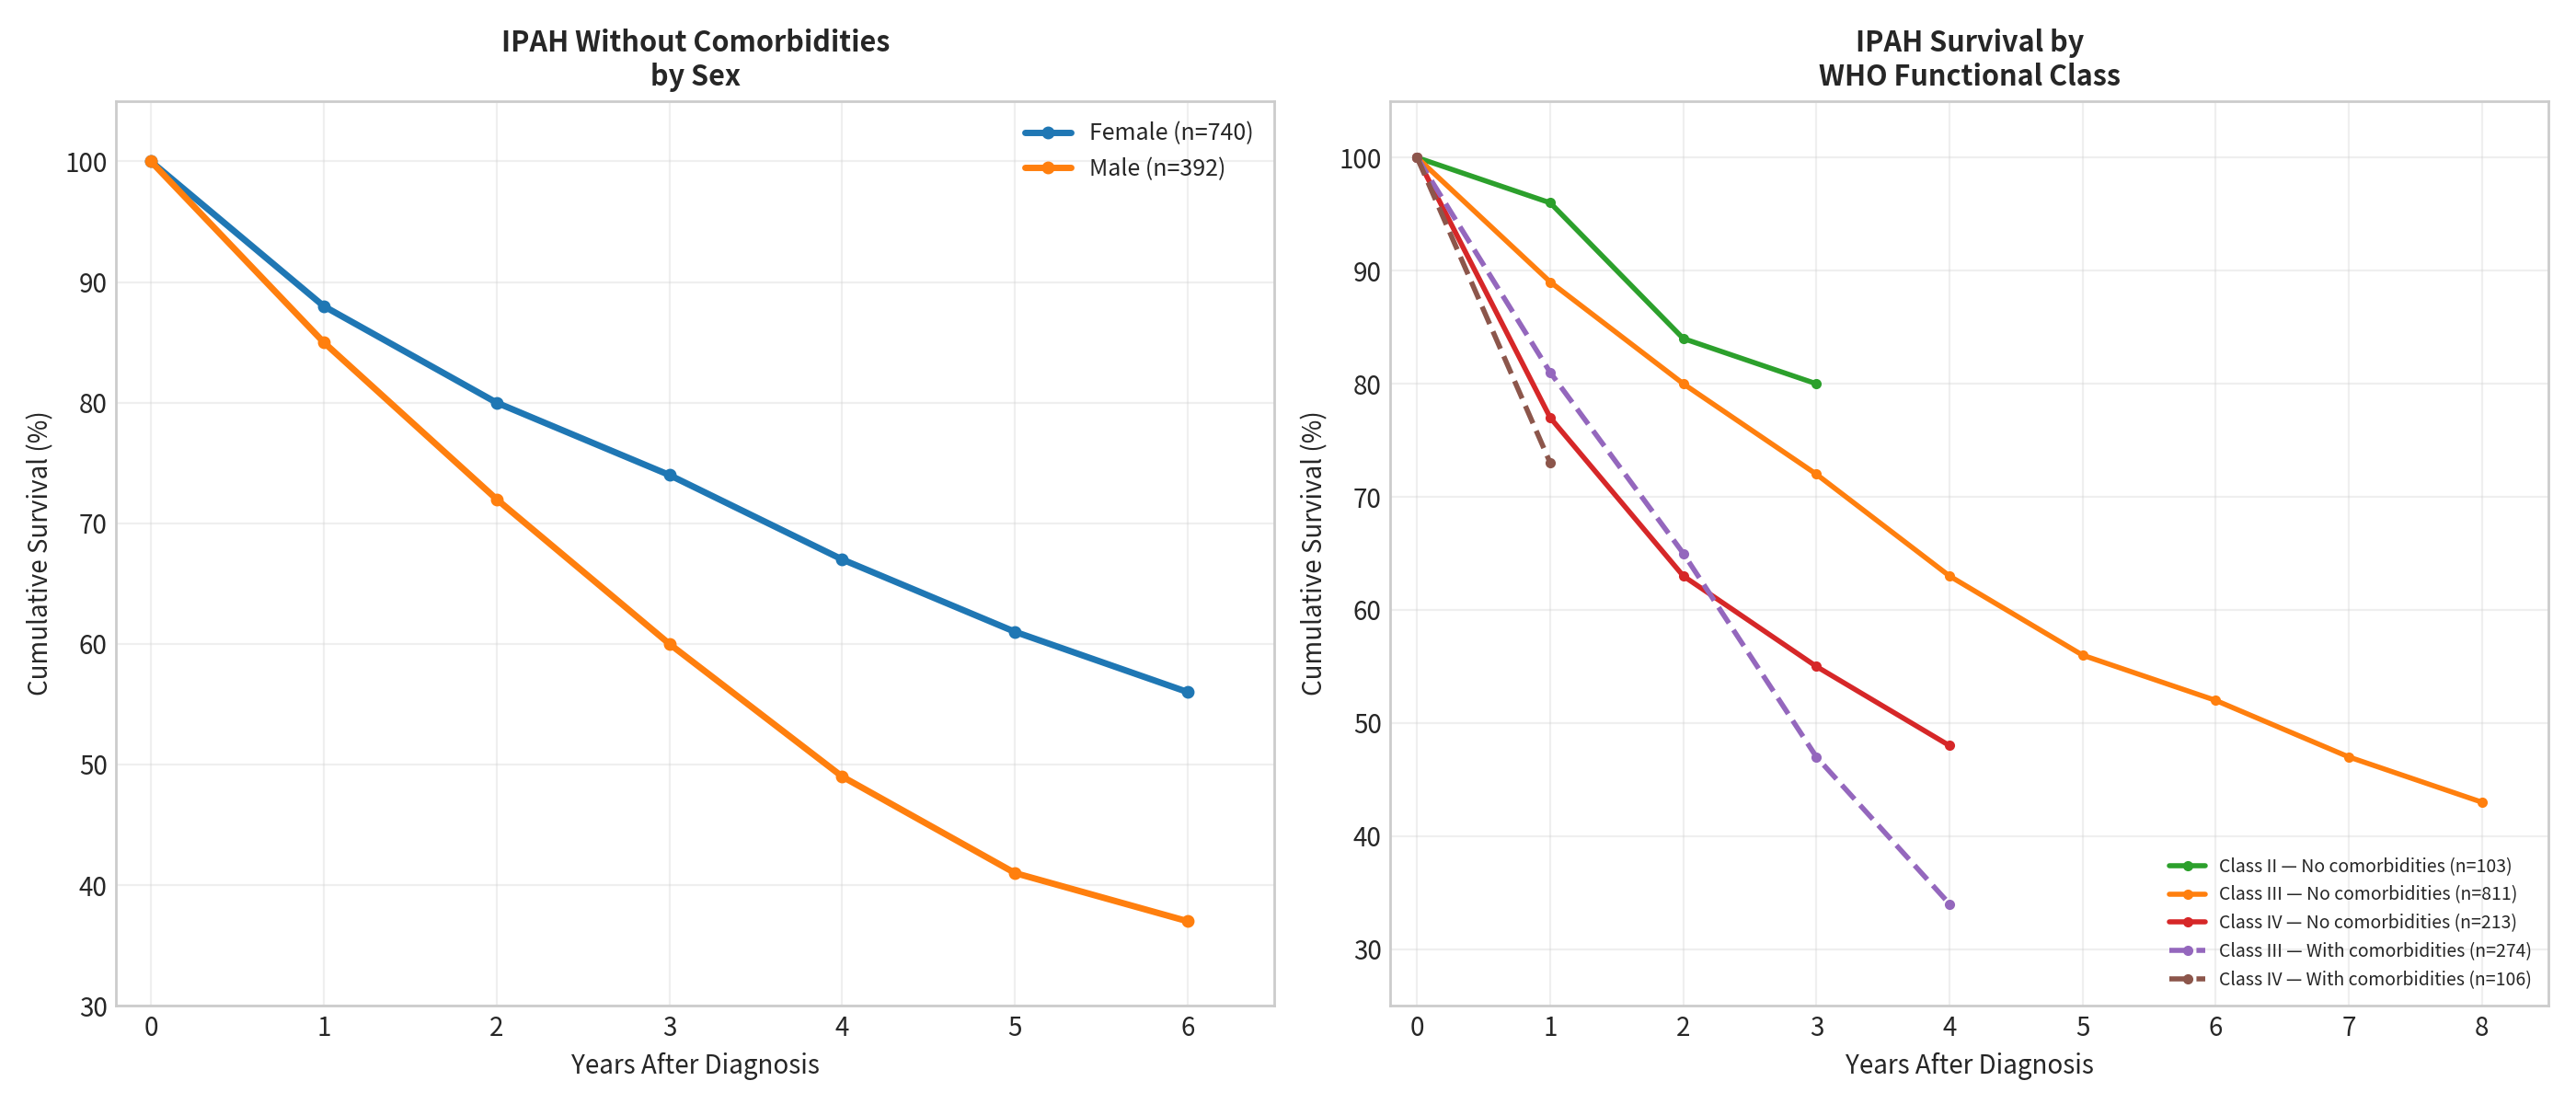
\includegraphics[width=\textwidth]{chart_survival_ipah_detailed.png}
  \caption{IPAH survival stratified by sex (left) and WHO functional class (right). Females without comorbidities survive longer than males (60\% vs 42\% at five years). WHO Class II patients maintain 80\% survival at three years, while Class IV patients fall to 48\% at four years. Comorbid patients fare worse at every functional class level.}
\end{figure}

Sex also modifies prognosis independently of age. Among IPAH patients without comorbidities, females (n=740) achieve 60\% five-year survival compared to 42\% for males (n=392). Female IPAH patients without comorbidities record the longest observed survival in any subgroup: 48\% at eight years, with 50\% mortality not reached at seven years and 77 days. Male IPAH patients with comorbidities face the steepest decline, reaching only 40\% at three years.

WHO functional class provides the most immediate prognostic signal at presentation. IPAH patients in WHO Class II (mild limitation) maintain 80\% survival at three years. Those in WHO Class III (marked limitation) drop to 72\% at three years and 43\% at eight years. WHO Class IV patients -- the most severely symptomatic -- average just 55\% survival at three years regardless of comorbidity status, with data too sparse beyond that point for precise estimation.

Drug prescribing patterns align with severity expectations. Combination therapy use has risen steadily from 25\% dual therapy and 3\% triple-plus in 2010 to 42\% dual and 5\% triple-plus in 2019, particularly among IPAH without comorbidities (57\% dual, 18\% triple-plus). Mono-therapy rates have declined from 72\% to 53\% across all patients. Sildenafil remains the dominant single agent (3,356 prescriptions in 2019, up from 1,518 in 2010), but macitentan has grown rapidly from zero to 1,139 as a newer endothelin receptor antagonist. Tadalafil similarly expanded from negligible use to 709 prescriptions. Riociguat and selexipag represent the newest additions, with 180 and 41 prescriptions respectively in 2019.

\begin{figure}[H]
  \centering
  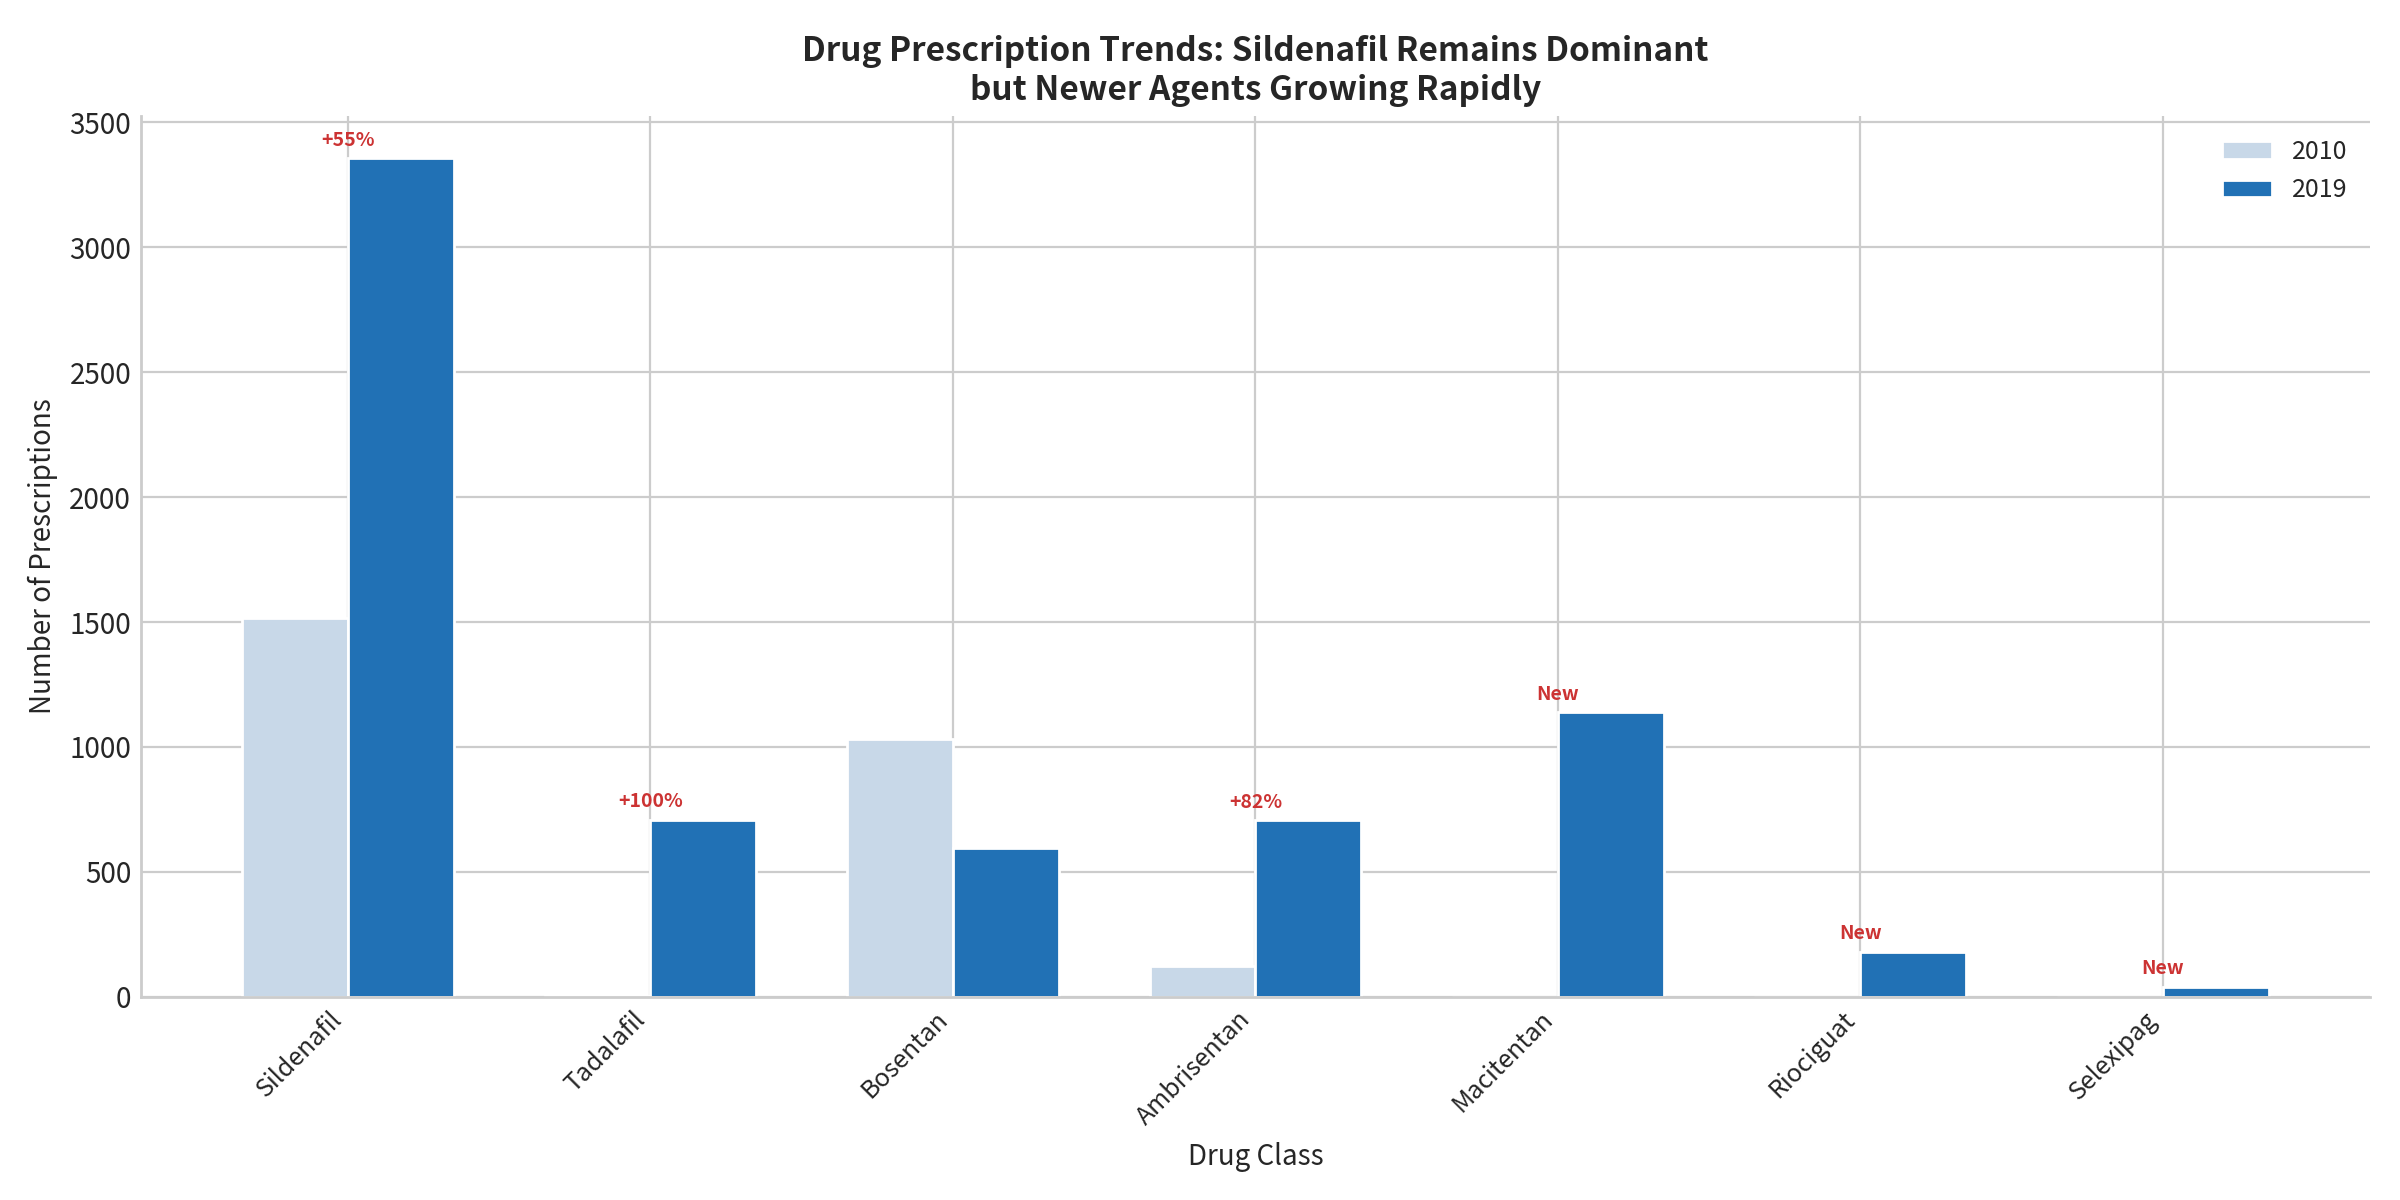
\includegraphics[width=\textwidth]{chart_drug_prescriptions.png}
  \caption{Drug prescription numbers changed dramatically between 2010 and 2019. Older agents like sildenafil remained popular but newer classes (macitentan, riociguat, selexipag) entered the market entirely. Bosentan usage declined significantly.}
\end{figure}

\section{Local action plans reveal targeted remediation strategies}

Five of the eight PH centres submitted explicit local action plans addressing national standards they failed to meet. The patterns of response differ meaningfully across organisations.

\textbf{Sheffield} acknowledged a decline in Standard 8 compliance (drug therapy within 12 weeks) from 87\% in 2016--17 to 79\% in 2018--19. Their remedy centres on workforce expansion: appointing a dedicated staff member to track patients through the pathway and adding a medical consultant in October 2019. They also undertook a service capacity review. For Standard 13 (PEA waiting times), Sheffield works with Royal Papworth, appointed an additional secretary to reduce administrative delays, assigned nursing staff to monitor the patient pathway, and is investigating coronary angiography wait times as a specific bottleneck.

\textbf{Golden Jubilee} similarly falls below the Standard 8 target at 61\% compliance. Their planned action focuses on increasing throughput for diagnostic right heart catheterisation, with stated confidence that the standard will be met in the next audit report.

\textbf{Newcastle} took a systems approach to Standard 3 (timely diagnosis), stating that Freeman Hospital monitors all new patient activity and works to ensure diagnoses are recorded within the recognised timeframe. They also noted improvements in Standard 8 following work on the 30-day target, rising from 33\% to 91\%.

\textbf{Imperial College} addressed Standard 5 differently -- their non-compliance stemmed from documentation errors rather than procedural failures. Cardiac catheterisations were performed externally but not correctly recorded in the database. Their remedy involves quarterly standard reviews to identify discrepancies closer to the time of entry.

\textbf{Royal Brompton and Harefield} adopted a proactive tracking strategy for Standard 13, continuing to monitor patients through the pathway, regularly auditing non-compliant cases, and aiming to adopt a virtual multidisciplinary team with Royal Papworth to shorten time to surgical suitability decisions.

The common thread across all responses is the recognition that patient pathway bottlenecks require dedicated staffing and process engineering -- not simply clinical guideline adherence. Administrative delays (secretaries, data entry, documentation), physical pathway monitoring (dedicated nursing staff), and cross-institutional coordination (virtual MDTs with Royal Papworth) emerge as recurring solutions.

\begin{figure}[H]
  \centering
  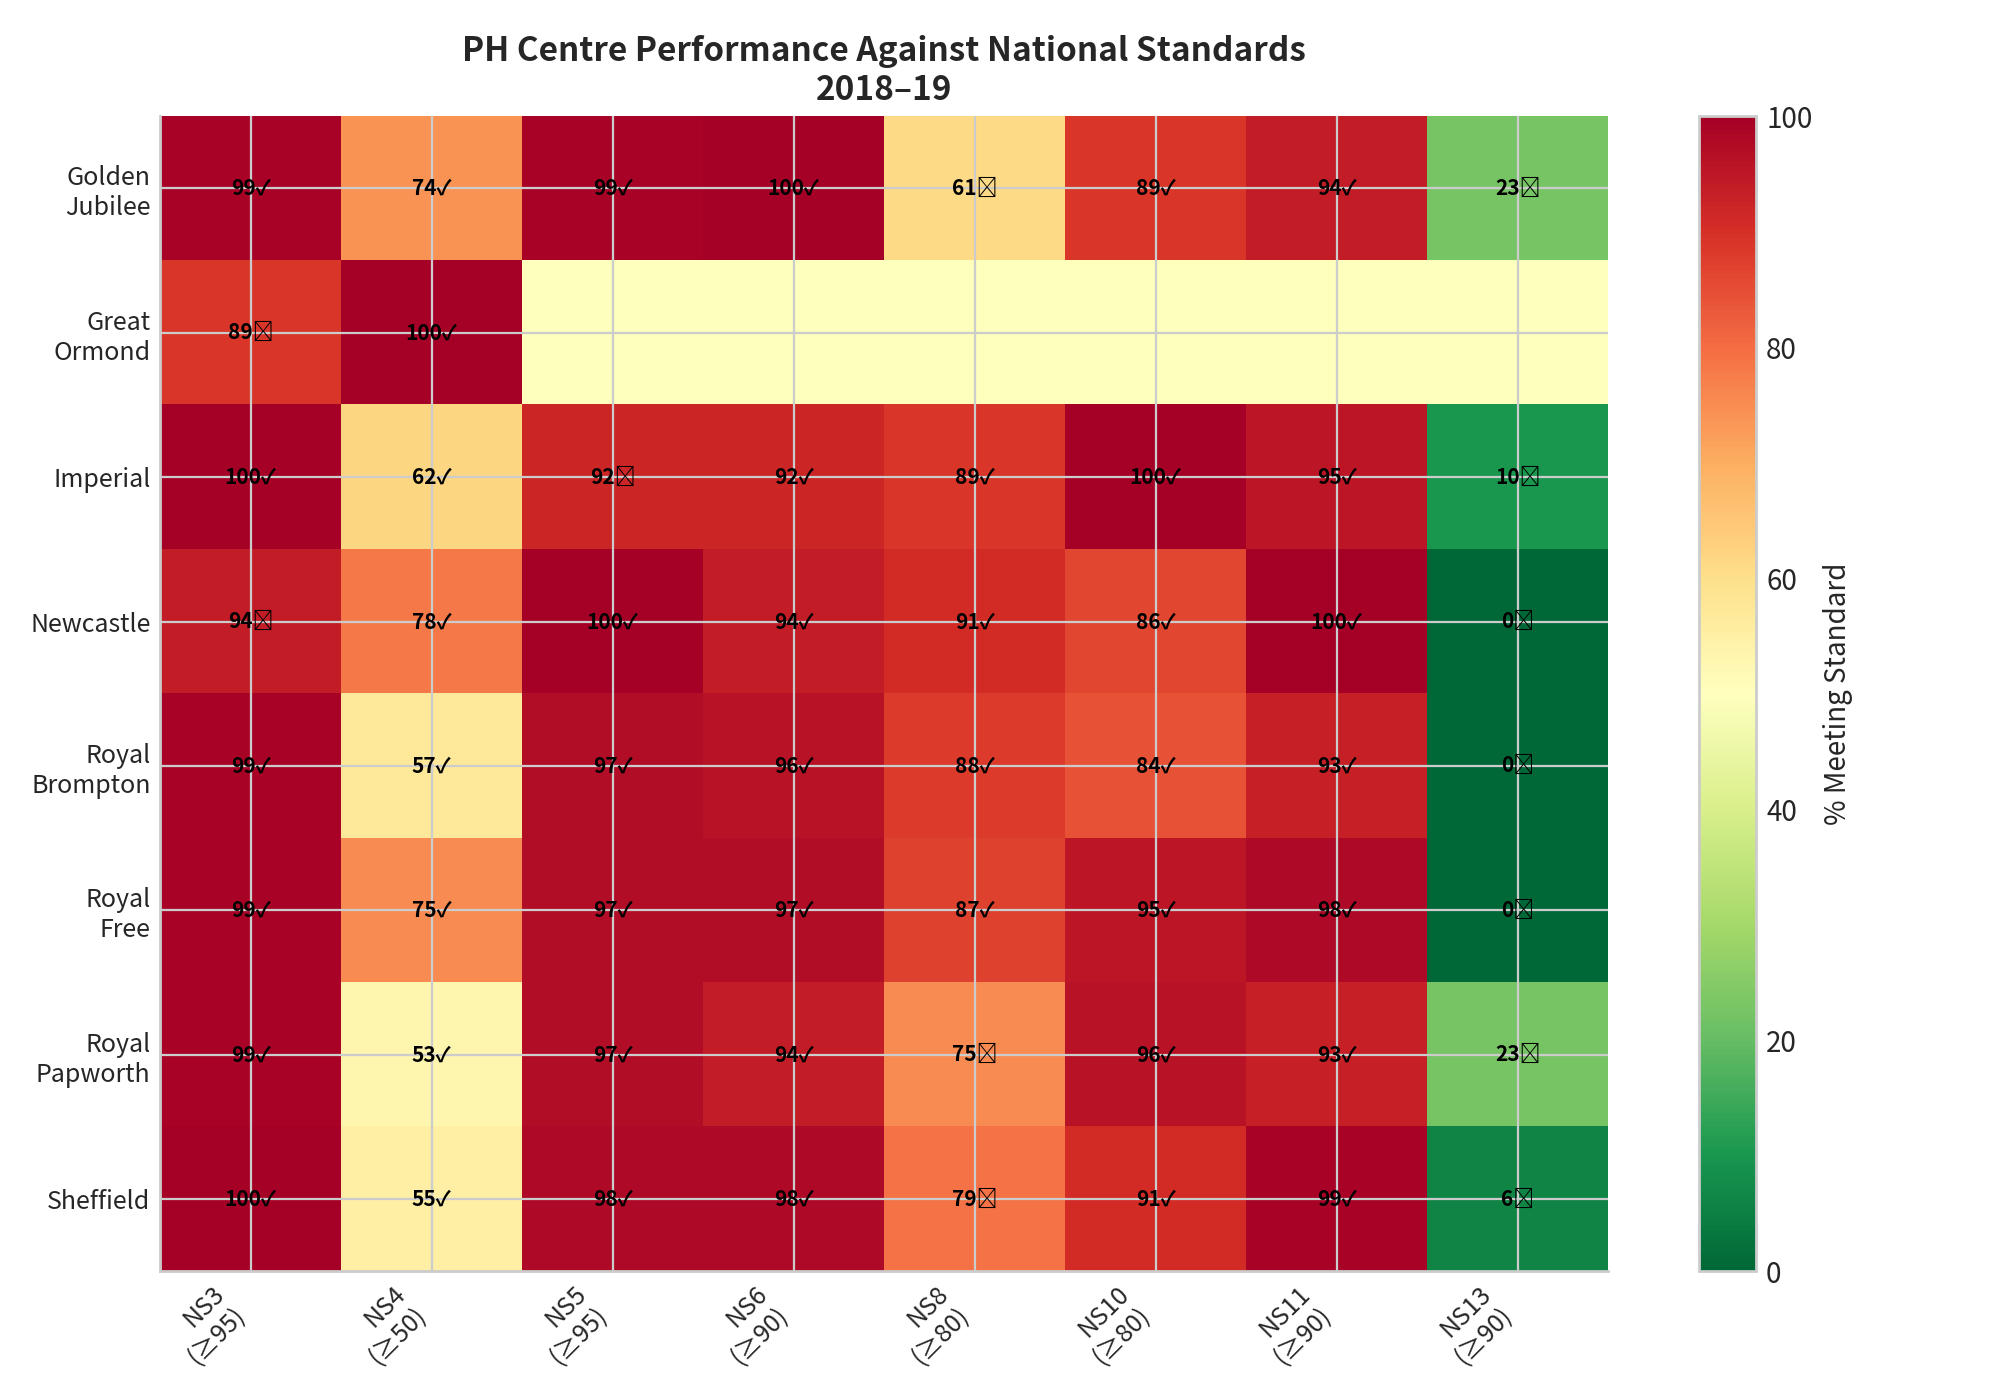
\includegraphics[width=\textwidth]{chart_centre_heatmap.png}
  \caption{Heat map of centre-level compliance across selected national standards. Green shades indicate达标 (meeting target); red indicates shortfall. Note that great Ormond Street and some metrics are N/A for certain centres. No centre meets all standards, highlighting persistent variation in care quality.}
\end{figure}

\section{Implications and next checks}

Several findings suggest priorities for the coming audit cycle. First, the PEA waiting time crisis demands attention. At 11\% national compliance against a 90\% target, Standard 13 is an outlier that no amount of internal process refinement can resolve without additional surgical capacity at Royal Papworth. Commissioner Kathy Blacker explicitly linked improvement to "increasing surgical capacity," and the move to Royal Papworth's new hospital is anticipated to address this constraint. Data should be monitored closely in the next report to confirm whether the relocation translates into reduced waiting times.

Second, vasoreactivity testing at 57\% compliance on a new 80\% standard requires embedding into routine practice. Centres should investigate whether the gap reflects equipment availability, specialist expertise, or documentation gaps -- distinguishing these categories will inform whether capital investment or training is the correct remedy.

Third, survival analysis by comorbidity status validates the clinical importance of the 2019 IPAH review. centres should continue maintaining the with/without comorbidities distinction in future reporting, as this classification explains vastly different outcome trajectories and prevents misleading aggregate survival estimates.

Fourth, Newcastle's dramatic Standard 8 improvement (33\% to 91\%) demonstrates that interventions targeting adjacent standards (like 30-day assessment) create positive spillover effects on downstream processes. Other centres falling short on Standard 8 might replicate this holistic pathway approach rather than treating each standard in isolation.

Limitations should be acknowledged: Scottish mortality data remains incomplete due to pseudonymisation protocols, which may slightly underestimate deaths in the aggregate longitudinal cohort. Patients treated across both English and Scottish centres may be counted twice. Survival curves truncate when fewer than 50 patients remain, potentially obscuring late-stage trends for smaller subgroups such as IPAH with comorbidities in older age quintiles or WHO Class IV with comorbidities. Finally, the rounding-up convention for standard compliance means some borderline percentages (e.g., 89.6\% rounded to 90\%) may appear compliant even though the underlying rate is nominally below target.

\bibliographystyle{plain}
\begin{thebibliography}{1}
\bibitem{naph10ar} National Audit of Pulmonary Hypertension, \emph{Great Britain, 10th Annual Report}, NHS Digital, 24 October 2019.
\bibitem{naph-supplement} National Audit of Pulmonary Hypertension, \emph{Supplementary Survival Analysis}, 24 October 2019.
\end{thebibliography}

\end{document}
